\documentclass{recipe}

\begin{document}
\begin{recipe}{Chicken, Biscuits, and Sprouts}
  \servings{3}

  \begin{ingredients}
    \ingredient{3}{}{chicken thigh}
    \ingredient{}{}{flour}
    \ingredient{}{}{paprika}
    \ingredient{}{}{salt}
    \ingredient{}{}{pepper}
    \ingredient{}{}{garlic powder}
    \ingredient{}{}{onion powder}
    \ingredient{5}{oz}{White Zinfandel}
    \ingredientsep
    \ingredient{24}{oz}{Brussles Sprouts}
    \ingredientsep
    \ingredient{4}{oz}{flour}
    \ingredient{1.25}{oz}{butter}
    \ingredient{}{}{milk}
    \ingredient{}{}{baking powder}
  \end{ingredients}

  \begin{images}
    \begin{image}
      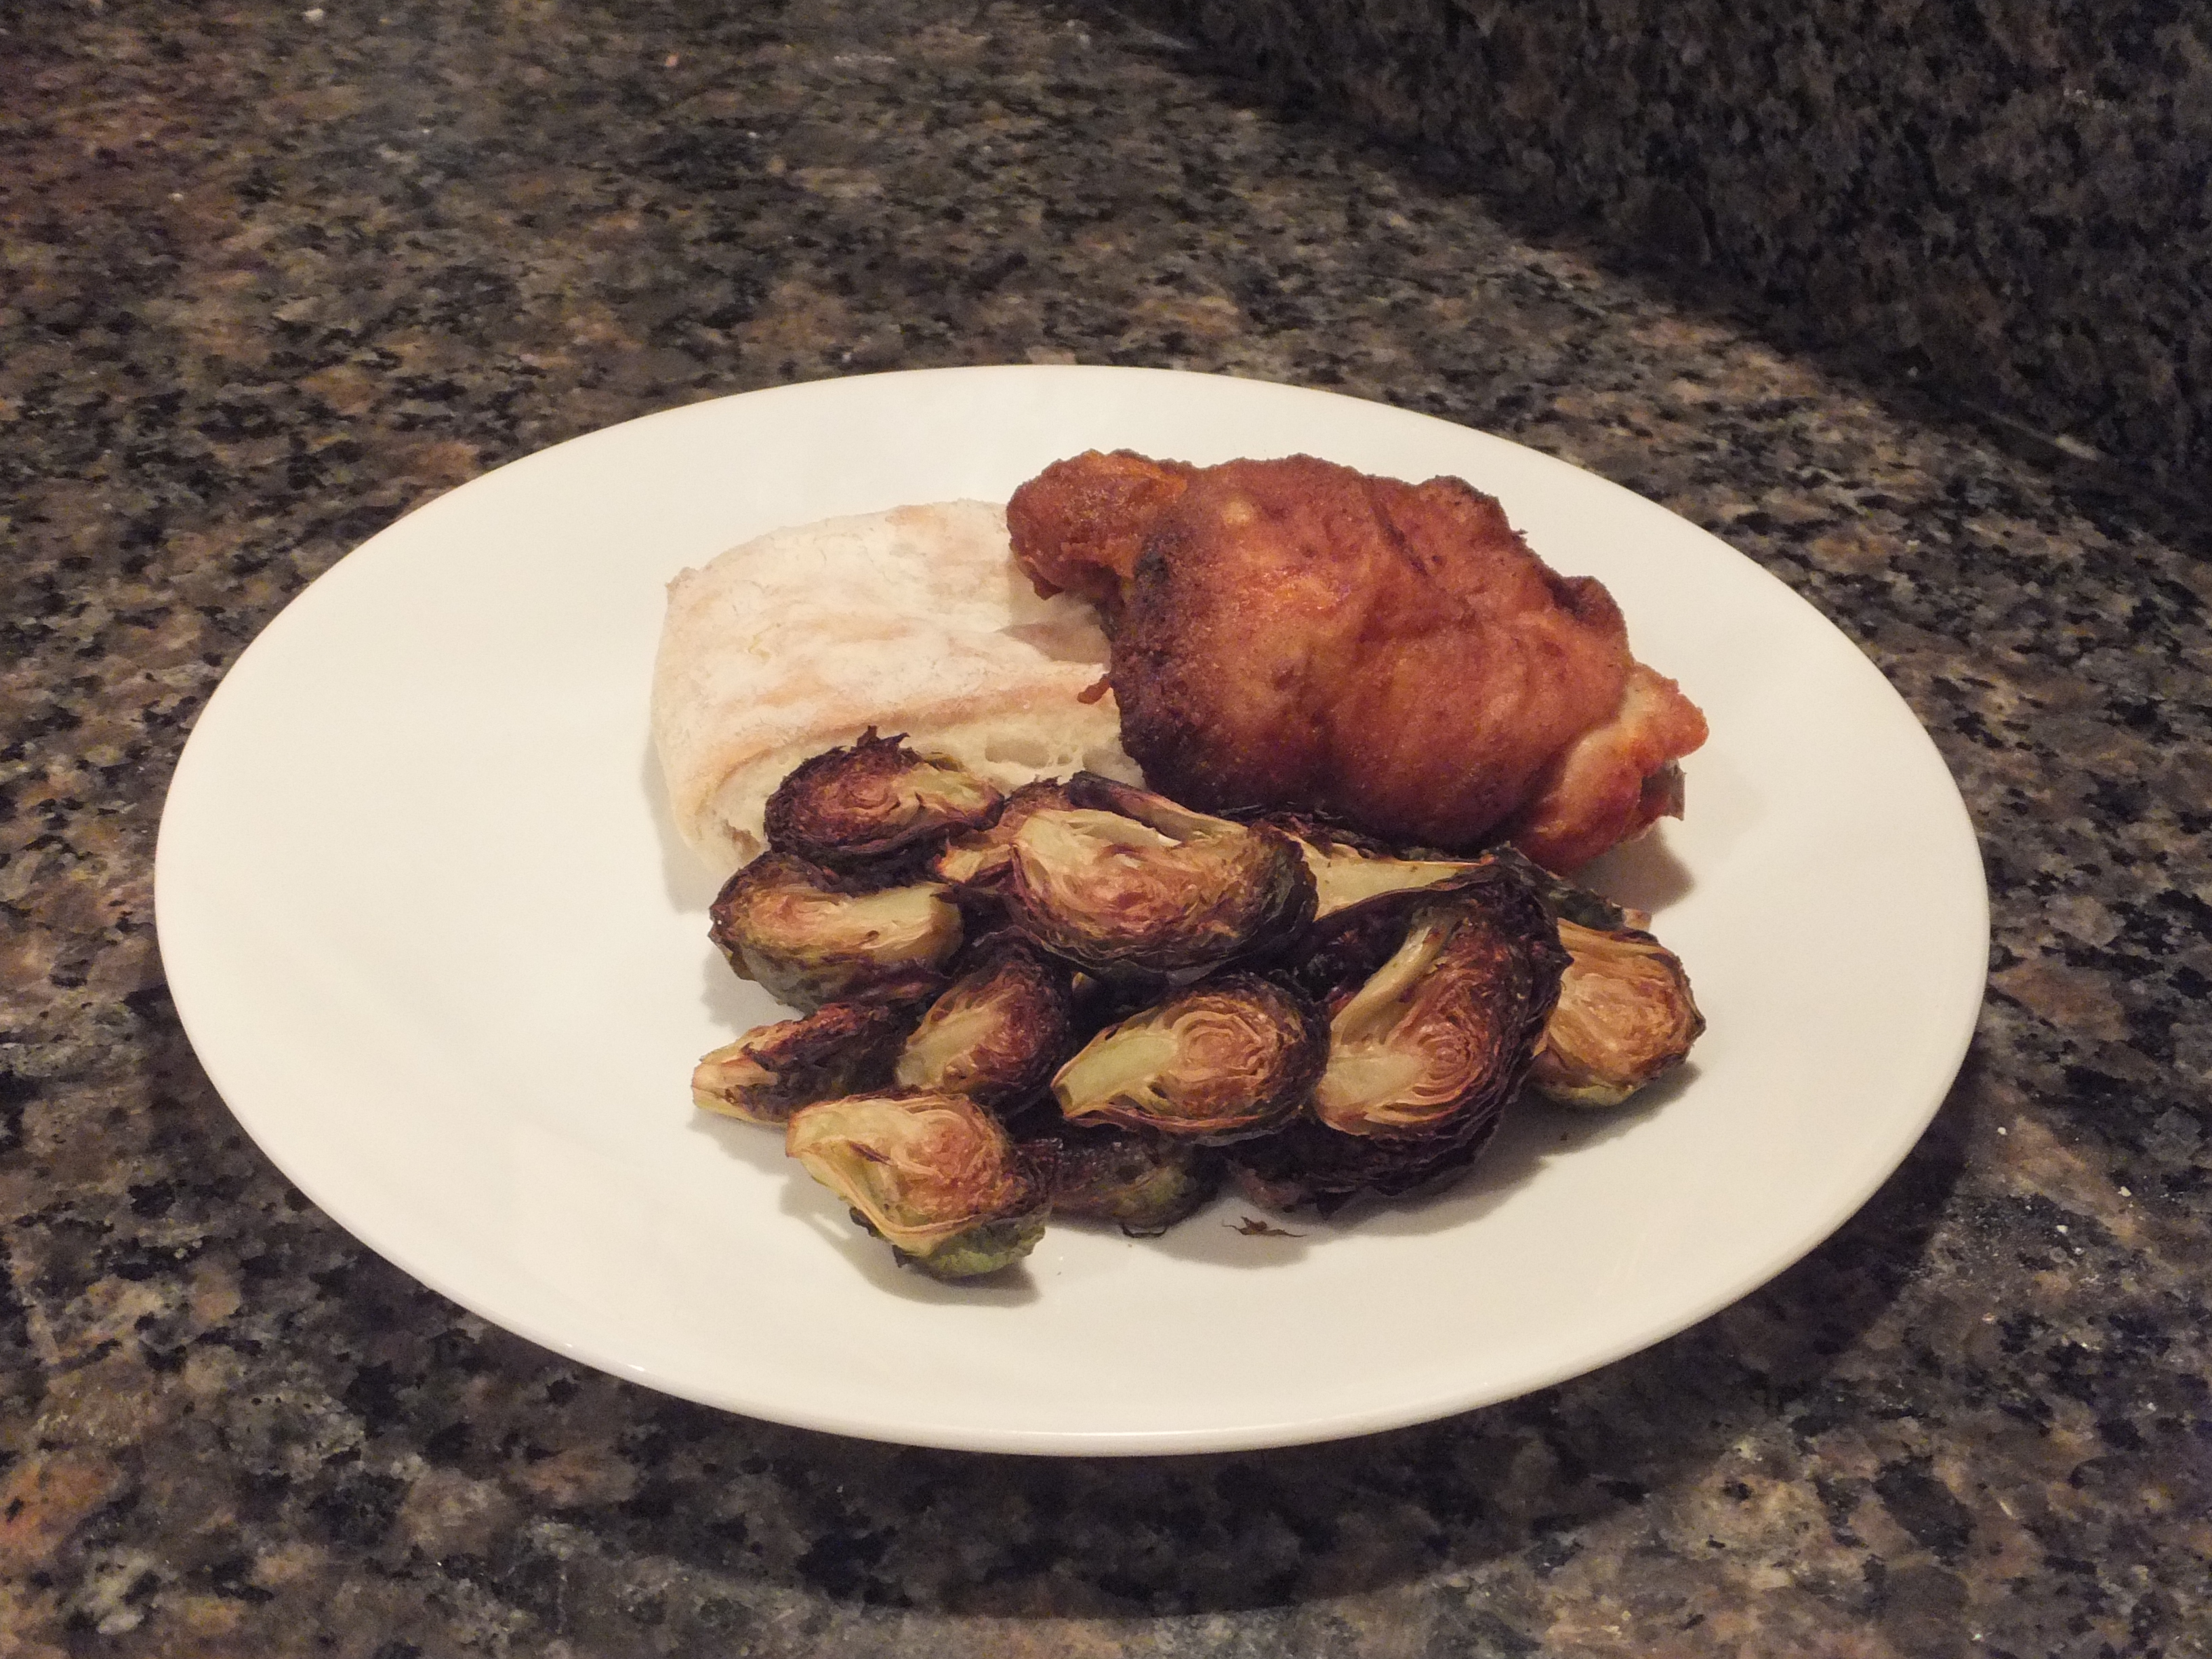
\includegraphics[width=\linewidth]{oven_fried_chicken-01.jpeg}
    \end{image}
  \end{images}

  \begin{steps}
  \item Trim and dry the chicken, particularly the skin side.
  \item Mix together all the spices with a bit of flour and coat the
    chicken with the rub.
  \item Place the chicken skin-side up on a baking rack.
  \item Bake the chicken at 450\degree F
  \item Cut the brussles sprouts in half and toss them with salt.
  \item Spread the vegetables on a baking sheet and spray the top side
    with oil.
  \item Add the vegetables to the oven
  \item Cut the butter into the bulk of the dry ingredients and then
    mix in the milk to barely make it come together.
  \item Fold the dough in thirds three times, creating a nice square
    block.  Cut this into biscuits and place in the oven in a greased
    baking dish for about 15 minutes.
  \item Remove the chicken to rest while making a sauce, continue
    cooking the vegetables and biscuits.
  \item Add the wine to the hot roasting pan to deglaze it, serve the
    chicken with the roasting juices, vegetables, and biscuits.
  \end{steps}

  \begin{notes}
  \item I think these should be roasted on top of some root vegetables to
    get a better sauce, last time it was too thin and acidic.
  \item Don't use that silly sweet wine (I tried because I didn't have
    vegetables, it didn't work at all!).
  \item I'm actually somewhat flip-floping on the wine issue, I boiled
    the sauce really hard for about 5 minutes and it turned out to be
    somewhat mellow in really small doses.  It might actually be worth
    eating...
  \end{notes}
\end{recipe}
\end{document}
